\documentclass{sigchi}
\usepackage{caption, subcaption, graphicx, url}

\newcommand{\strong}[1] {\textbf{#1}}
\newcommand{\code}[1] {\texttt{#1}}

\begin{document}
\title{Evidence for Autosuggest for Syntactic Search}
\numberofauthors{2}
\author{
  \alignauthor 1st Author Name\\
    \affaddr{Affiliation}\\
    \affaddr{Address}\\
    \email{e-mail address}
  \alignauthor 2nd Author Name\\
    \affaddr{Affiliation}\\
    \affaddr{Address}\\
    \email{e-mail address}
}


\maketitle

\begin{abstract}
%!TEX root = chi14grammatical.tex

A common task in qualitative data analysis is to characterize the usage of a word or concept. The ability to issue queries over syntactic relations between words is useful in these situations, as it allows users to see other words that have significant relationships with a query word. Previous interfaces for  searching over syntactic structures require programming-style queries and formal linguistic terminology, but expertise in these fields is scarce. Interfaces for non-experts must therefore be able to show options for searching for different syntactic relations in ways that allow the user to recognize the relation that is being queried. We therefore investigated how to present syntactic relations between words in a recognizable way. An experiment with 400 participants found that syntactic relations are recognized with 34\% higher accuracy when contextual examples are shown, than a baseline of naming the relations alone.  This indicates that more user-friendly query interfaces for syntactic search should augment the shown options with contextual examples.

\end{abstract}

\keywords{Search, Syntax, Grammatical Queries, Digital Humanities, Information Extraction}

\category{H.5.m.}{Information Interfaces and Presentation (e.g. HCI)}{Miscellaneous}

\section{Introduction}
%!TEX root = chi14grammatical.tex
%What does $X$ do? How is $Y$ described? Most analysts and researchers ask themselves these questions while trying to understand a subject.  So far, the field of information retrieval has tackled this problem indirectly: the analyst enters a search query, and the system returns some results. When the underlying data has structure, queries can be specific and targeted -- and there is now a substantial body of work [cite] on how best to issue structured queries over \emph{structured} data. But what if the ``data" is is text -- medical literature, legal records, interview transcripts? Although text is richly structured by rules of  grammar and narrative, it is rarely treated as such. While there is a lot of work on extracting various kinds of structured information from text, there is little on how to make it easy for users to access and query over it.  As the questions above show, however, structured queries over language can be extremely useful. In grammatical terms, they become ``What are the verbs of which $X$ is the subject?'' ``What are the adjectives that modify $Y$?''
%
%Adapting existing structured-query interfaces to grammatical search is problematic for several reasons. The first is that the structures in language are not explicit, like columns in a table, but are implicit, and have to be extracted computationally. Only in the last decade have computational linguistic technologies become fast and accu rate enough to use in the real world.
%
%The second problem is the lack of programming experience among searchers. Current structured query languages like SPARQL have complex syntaxes that require time and effort to learn. For example, here is a SPARQL query for ``What are all the country capitals in Africa?'':
%\begin{verbatim}
%SELECT ?capital ?country
%WHERE {
%  ?x cityname ?capital ;
%     isCapitalOf ?y .
%  ?y countryname ?country ;
%     isInContinent Africa .
%}
%\end{verbatim}
%Even if we assume that only professional analysts engaging in information-intensive work would want to issue such targeted queries,  programming experience is scarce. One study on a query language for selecting phrase structures from sentences found that that only 50\% of the people who wanted to use it had programming experience \cite{}.
%
%The third problem is that there are no common-language terms for grammatical relationships even though ordinary people are perfectly capable of understanding and using them. Modern parsers use standard linguistics terminology to label their outputs, but those technical names and definitions are not always accessible to those outside the field. Take the phrases ``he threw the ball" and ``the ball was thrown by him". In both cases, it is clear that `he' is is the one who `threw' whereas, in grammatical terms, the first phrase is in the active case, and the phrase is in the passive case. The Stanford Dependency Parser \cite{}, for example, outputs two different variants of the verb-subject relation: \code{nsubj(he, threw)} and \code{nsubjpass(he, threw)}. A grammatical search system therefore has to bridge the gap between the relations that are recognizable to people and the relations that are extracted from the data

Web search engines are effective for keyword searches and (increasingly) natural language queries, but intuitive interfaces are still lacking for  syntactically structured queries such as \emph{ find all adjectives that modify ``clothes"}. Such queries are useful in the humanities and social sciences, when scholars attempt to characterize concepts, and also in the field of information extraction for developing complex patterns for recognizing entities in text, such as medical terms \cite{hirschman2005overview,maclean2013identifying}, and  products and organizations \cite{culotta2005reducing}.

Our goal is to build interfaces to help humanities scholars search and analyze written literature; however, according to a recent large survey \cite{gibbs_building_2012}, this group is often skeptical of digital tools, primarily because they are often difficult to use.  A different survey found that  linguists wished to make very technical  linguistic queries, but 55\% of them did not know how to program \cite{soehn2008requirements}. Despite this, most existing interfaces for  querying syntactically structured text require complex program-like syntax, reducing the likelihood that the target users will be willing or able to use the tool.

To address this gap, we conducted an experiment to investigate how grammatical relationships between English words can be made more recognizable to ordinary people. Following the principle of recognition over recall, as well as the success of auto-suggest in search query interfaces, we hypothesized that examples would help people identify grammatical relationships more accurately than technical names.

Our results confirm that showing examples in the form of words or phrases that match significantly improves the accuracy with which grammatical relationships are recognized over a standard baseline.  Our findings also showed that different types of relations benefited differently depending on how much context was shown in the auto-suggest examples.

These findings suggest that a query interface in which a user enters a word of interest and the system shows candidate grammatical relations augmented with examples from the text will be more successful than the baseline of simply naming the relation and showing gaps where the participating words appear.


%In a follow-up experiment, we found that if distinctive or closed-class words tend to participate in a grammatical relationship, then a list of matching words is the best recognition aid. By contrast, in clausal or long-distance relationships, where the context determines how the two words are related, a list of phrases is best.

%The rest of this paper is structured as follows. In the next section, we summarize the previous work on issuing structured queries over linguistic information extracted from text data. Then, we  describe our experiments and analyze the results. Finally, we summarize our findings and discuss their implications for grammatical search interfaces.


%!TEX root = chi14grammatical.tex

\section{Related Work}

Because trees are the traditional representation of a syntactic parse, some  tools that allow querying of  collections of syntactically parsed data focus on tree structures.   For instance, the Linguist's Search Engine \cite{resnik2005web} uses a query-by-example strategy in which a user types in an initial sentence in English, and the system produces a graphical view of a parse tree as output, in addition to a nested LISP expression of the same tree.  The user can either click on the tree or modify the LISP expression to generalize the query.    Similarly, the popular Stanford Parser includes Tregex, which as the name suggests,  allows for sophisticated regular expression search over syntactic tree structures, and Tsurgeon, which allows for manipulation of the trees extracted with Tregex \cite{levy2006tregex}.  Neither of these tools have been evaluated with usability studies.  The Finite Structure Query tool for querying syntactically annotated corpora requires its queries to be stated in first order logic \cite{kepser2003finite}. In the Corpus Query Language \cite{jakubicek2010fast}, a query is a pattern of attribute-value pairs.

Another approach (discussion of XML, Sparql goes here.)

A final simple alternative approach is to simply name the relation of interest and show blanks where the words that satisfy the relation would appear; this is the baseline design tested below.

According to Shneiderman and Plaisant \cite{shneiderman2010designing}, query-by-example has largely fallen out of favor as a user interface design approach.  At the same time, a related technique, auto-suggest, has become a widely-used approach in search user interfaces with strong support in terms of its usability \cite{hearst2009search}.  More here...

\section{Experiment 1: do Examples Help?}
%!TEX root = chi14grammatical.tex


Our goal was to find out whether showing examples improves the recognizability of grammatical relations. We tested two types of examples: a list of matching words and a list of matching phrases. Words are explicitly visible in the text, but phrases provides contextual information that helps determine the relationship.

Our hypothesis was:
\begin{quote}
	H1. Grammatical relations are identified more accurately when shown with examples of contextualizing words or phrases than without.
\end{quote}

To test H1, participants were given a series of identification tasks. In each task, they were shown a list of 8 sentences, each containing a particular relationship between highlighted words. They were asked to identify the relationship from a list of 4 choices.  Additionally, one word was chosen as a \emph{focus word} that was present in all the sentences, to make the relationship more recognizable (``life'' in Figure~\ref{fig:choices}).

The choices were displayed in 3 different ways (Figure \ref{fig:choices}).  The \strong{baseline} presentation
(Figure \ref{fig:baseline-choices}) named the linguistic relation and showed a blank space with a peach background for the varying word in the relationship, the focus word highlighted in yellow and underlined, and any necessary additional words necessary to convey the relationship (such as ``of" for the prepositional relationship containing ``of",  the third option).

The \strong{words} presentation showed the baseline design, and in addition beneath it showed the word ``Examples:'' followed by a list of 4 example words that could fill in the peach-colored blank slot (Figure \ref{fig:words-choices}).   The \strong{phrases} presentation again showed the baseline design, beneath which was shown the phrase ``Patterns like:'' and a list of 4 example phrases in which fragments of text including both the peach and the yellow highlighted portions of the  relationship appeared (Figure \ref{fig:task}).

We used a between-subjects design. The task order and the choice order were not varied: the only variation between participants was the presentation of the choices. To avoid the possibility of participants guessing the right answer by pattern-matching, we ensured that there was no overlap between the list of sentences shown, and the examples shown in the choices as words or phrases. Not every relationship shown in the distractors was tested, and distractors were chosen to be ones intuitively most likely to be mistaken for  the relationship shown.

The tasks were generated using the Stanford Dependency Parser \cite{de2006generating} on the text of \emph{Moby Dick} by Herman Melville. We tested the 12 most common grammatical relationships in the novel in order to cover the most content and to be able to provide as many real examples as possible. These relationships fell into two categories:.


Clausal or long-distance relations:
	\squishlist
		\item \strong{advcl} Adverbial clause: \emph{ I \textbf{walk} while \textbf{talking}}
		\item  \strong{xcomp} Open clausal complement:  \emph{I \textbf{love} to \textbf{sing} }
		\item  \strong{ccomp} Clausal complement:  \emph{ he \textbf{saw} us \textbf{leave}}
		\item  \strong{rcmod} Relative clause modifier:  \emph{the \textbf{letter} I \textbf{wrote} reached }
	\squishend

Other relations:
		\squishlist
			\item \strong{nsubj} Subject of verb: \emph{\textbf{he} \textbf{threw} the ball}
			\item \strong{dobj} Object of verb:  \emph{ he \textbf{threw} the \textbf{ball}}
			\item \strong{amod} Adjective modifier \emph{\textbf{red} \textbf{ball}}
			\item \strong{prep\_in}  Preposition (in): \emph{a \textbf{hole} in a \textbf{bucket}}
			\item \strong{prep\_of}	Preposition (of):  \emph{ the \textbf{piece} of \textbf{cheese}}
			\item \strong{conj\_and}  Conjunction (and)  \emph{ \textbf{mind} and \textbf{body}}
		\item\strong{advmod} Adverbial modifier: \emph{  we \textbf{walk} \textbf{slowly}}
		\item \strong{nn} Noun compound:  \emph{ \textbf{Mr.}  \textbf{Brown}}
	\squishend

We tested each of the above relations 4 times, with 2 different focus words in each role. For example, the verb-subject relation \code{nsubj} was tested in the following forms:
\squishlist
	\item \code{nsubj(Ahab, \_\_\_)}:  the sentences each contained `Ahab', highlighted in yellow, as the subject of different verbs highlighted in peach.
	\item \code{nsubj(captain, \_\_\_)}

	\item \code{nsubj(\_\_\_, said)}: the sentences all contained the verb `said', highlighted in yellow, but with different subjects, highlighted in peach.
	\item \code{nsubj(\_\_\_, stood)}
\squishend

To maximize coverage, yet keep the total task time reasonable (average 6.8 minutes), we divided the relations above into 4 task sets of 3 relations each. Each relation was tested with 4 different words, making a total of 12 tasks per participant.

\subsection{Participants}
Participants were paid 50c (U.S.) for completing the task, with an additional 50c bonus if they correctly identified 10 or more of the 12 relationships. They were informed of the possibility of the bonus before starting the task.

To help ensure the quality of effort from participants, we included a multiple-choice screening question, `What is the third word of this sentence?"  Those that answered incorrectly were eliminated. 400 participants completed the study distributed randomly over the 4 task sets and the 3 presentations. To gauge their syntactic familiarity, we also asked them to rate how familiar they were with the terms `adjective' (88\% could define it), `infinitive' (43\%), and `clausal complement' (18\%).

\subsection{Results}
\begin{figure}
\centering
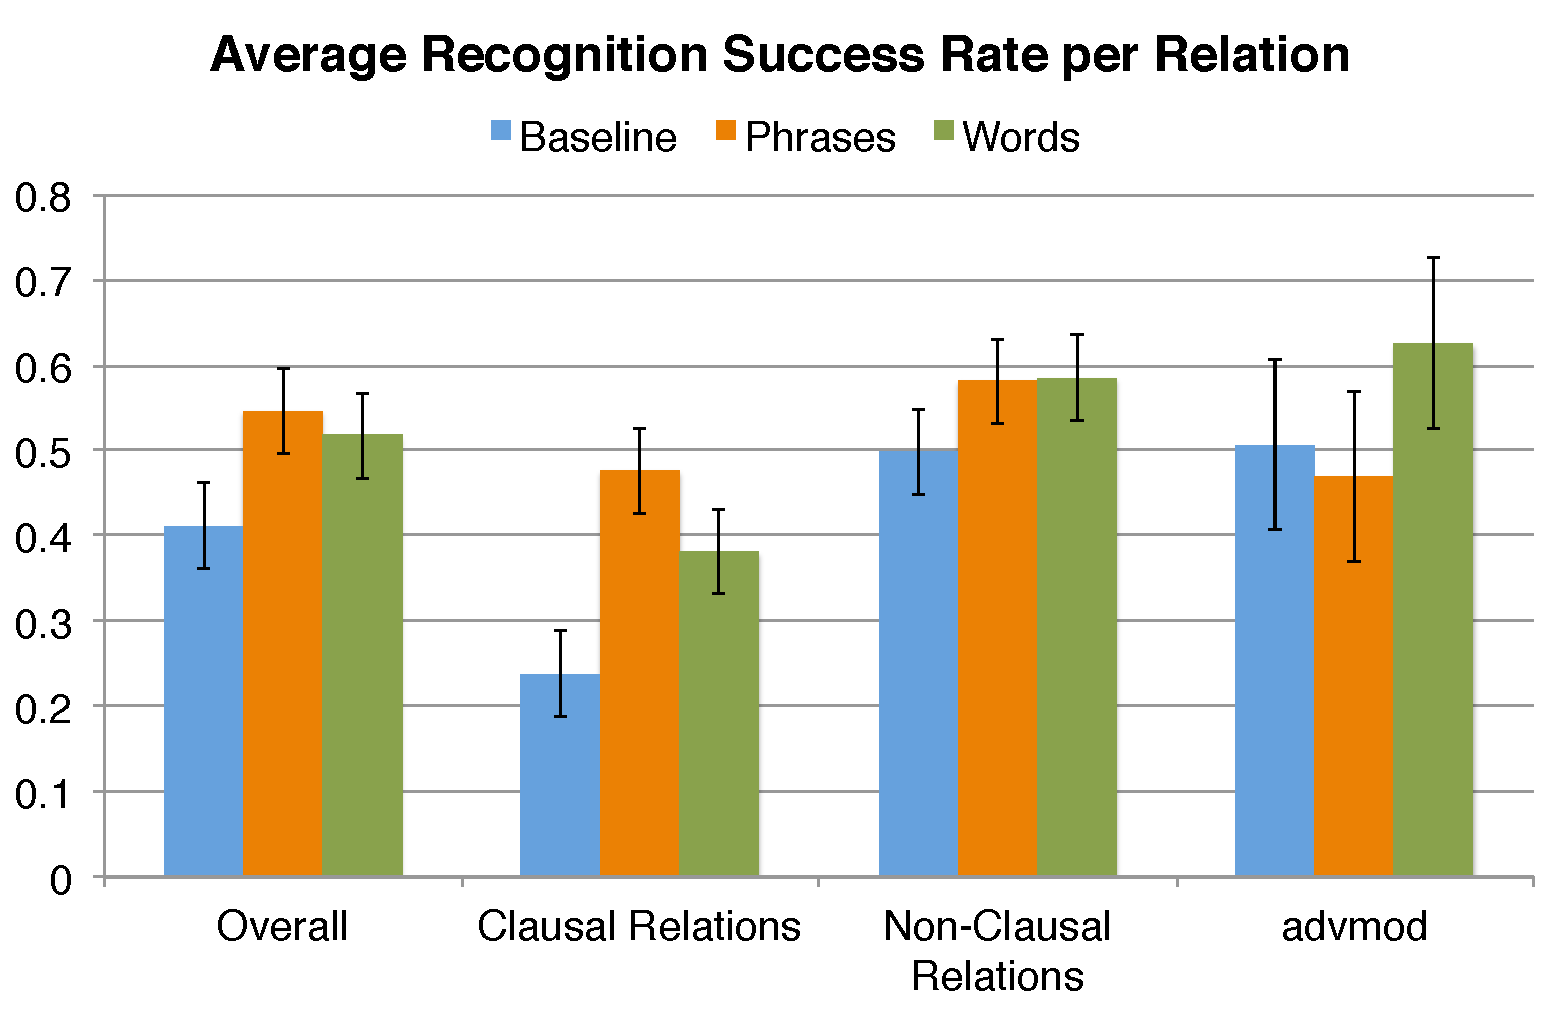
\includegraphics[width=\columnwidth]{fig/results}
\caption{\label{fig:results} Recognition rates for different types of relations under the 3 experiment conditions, with 95\% confidence intervals.}
\end{figure}

The results (Figure \ref{fig:results}) confirm H1. Participants in conditions that showed examples (\strong{phrases} and \strong{words}) were significantly more accurate at identifying the relations than participants in the \strong{baseline} condition. We used the Wilcoxson signed-rank test, an alternative to the standard T-test that does not assume samples are normally distributed. The average success rate in the \strong{baseline} condition was $41\%$, which is significantly less accurate than \strong{words}: $52\%, (W = 6136, p = 0.00019)$, and \strong{phrases}: $55\%, (W = 5546.5, p = 0.00014)$.


Clausal relations operate over longer distances in sentences, and so it is to be expected that showing longer stretches of context would perform better in these cases; that is indeed what the results showed.
Phrases significantly outperformed words and baseline. The average success rate was 48\% for \strong{phrases}, which is significantly more than \strong{words}: 38\%, (p = 0.017) and \strong{baseline}: 24\%, ($p= 1.9 \times 10^-9$), which was indistinguishable from random guessing (25\%). This is a surprisingly strong improvement, given that only 18\% of participants reported being able to define  `clausal complement'.

For the non-clausal relations, there was no significant difference between \strong{phrases} and \strong{words}, although they were both overall significantly better than the baseline (words: $p=0.0063$, phrases: $p=0.023$). Among these relations, adverb modifiers (\code{advmod}) stood out (Figure \ref{fig:results}), because evidence suggested that \strong{words} (63\% success) made the relation more recognizable than \strong{phrases} (47\% success, $p = 0.055$) -- but the difference was only almost significant, due to the smaller sample size (only 96 participants encountered this relation). This may be because the words are the most salient piece of information in an adverbial relation -- adverbs usually end in `ly' -- and in the phrases condition the additional information distracts from recognition of this pattern.



\section{Discussion}
%!TEX root = chi14grammatical.tex


The results imply that auto-suggest interfaces for syntactic search should show candidate relationships augmented with a list of phrases in which they occur. A list of phrases is the most recognizable presentation for clausal relationships (34\% better than the baseline), and is as good as a list of words for the other types of relations. A mockup of such a search interface is shown in Figure \ref{fig:phrases-mockup}.  Selecting the choice will return all sentences that contain the search term and match the relation.
\begin{figure}
\centering
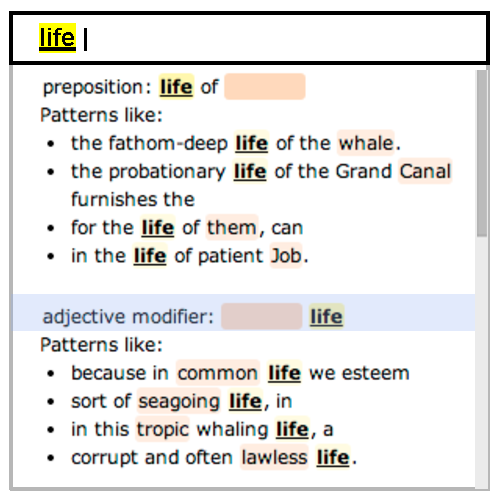
\includegraphics[width=0.5\columnwidth]{fig/phrases-mockup}
\caption{
	\label{fig:phrases-mockup} Mockup of auto-suggest for syntactic search on the word `seen', showing clausal relations with example phrases.
}
\end{figure}

There is a tradeoff between recognizability and space required for scrolling through the choices, although it is important to keep in mind that because the suggestions are populated with phrases from the collection itself, they are informative.    Further, the suggestions can be ordered by frequency of occurrence in the collection, or by an interestingness measure given the search word.  As the user becomes more familiar with a given relation, it may  be expedient to shorten the cues shown, and then re-introduce them if a relation has not been selected after some period of time as elapsed.

The best  strategy, \strong{phrases}, had an overall success rate of only 55\%, although the intended user base may have more familiarity with grammatical relations than the participants did, and therefore may perform better in practice.  Nonetheless, there is room for improvement in scores, and it may be that additional visual cues, such as some kind of bracketing, will improve results.  Furthermore, the current study did not test three-word relationships or more complex combinations of structures, and those may require improvements to the design.


\bibliographystyle{acm-sigchi}
\bibliography{papers}

\end{document}


%\section{Experiment 2}
%We hypothesized that words were more helpful when the relations involved distinctive or closed-class words: adverbs are distinctive because they usually end in `ly' -- thoughtfully, helpfully, quickly, etc. Closed-class words include determiners (a, the, that, etc.), pronouns and prepositions.  Our follow-up hypothesis was:
%
%\begin{quote}
%	H2. If distinctive or closed-class words enter into a grammatical relation, then showing a list of matching words makes it easier to recognize the relation. In other cases, a list of example phrases is more helpful.
%\end{quote}
%
%We conducted a follow-up study to verify this hypothesis. This study was had the same design as the first study: a series of identification tasks in which there was a query word and a relationship. The participants  were shown a list of sentences containing that relationship between the query word and other words, their task was to identify which relationship it was, from a list of 4 choices. Except this time, instead of presenting all the choices in the same way (as a list of matching words, or a list of matching phrases) we presented each choice in the way we thought would be most useful according to our hypothesis. If the hypothesis was true, participants in this `optimal presentation' condition would outperform participants who had all the options presented in the same way.
%
%The results from this follow-up experiment  confirmed our hypothesis.
